\documentclass[border=10pt]{standalone}
\usepackage{pgfplots}
\pgfplotsset{compat=1.18}
\begin{document}
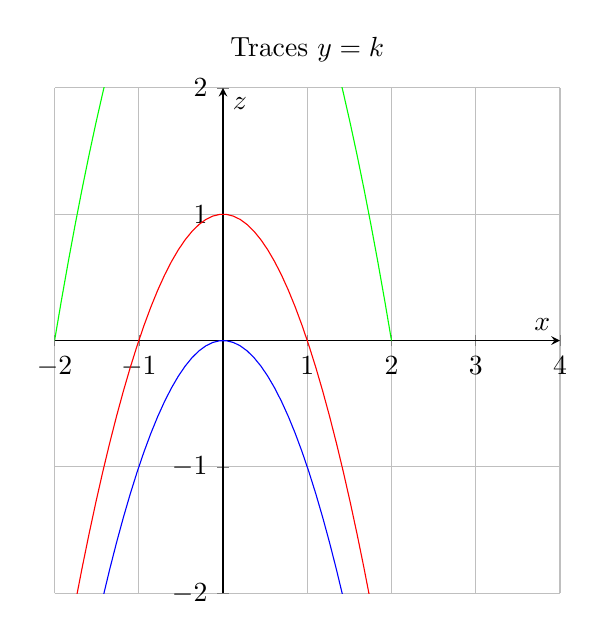
\begin{tikzpicture}
\begin{axis}[
    xlabel={$x$},
    ylabel={$z$},
    title={Traces $y=k$},
    xmin=-2, xmax=4,
    ymin=-2, ymax=2,
    axis lines=center,
    grid=major,
    width=8cm,
    height=8cm,
]
% y=0: x = -z^2
\addplot[blue, domain=-2:2, samples=50] {-x^2};
% y=1: x = 1-z^2
\addplot[red, domain=-2:2, samples=50] {1-x^2};
% y=2: x = 4-z^2
\addplot[green, domain=-2:2, samples=50] {4-x^2};
\end{axis}
\end{tikzpicture}
\end{document}